\documentclass[a4paper]{article}

\usepackage[english]{babel}
\usepackage[utf8x]{inputenc}
\usepackage{amsmath}
\usepackage{amsfonts}
\usepackage{graphicx}
\usepackage{hyperref}
\usepackage[colorinlistoftodos]{todonotes}

\title{CS 5785 -- Applied Machine Learning -- Lec.\ 11}
\author{Prof.\ Nathan Kallus, Cornell Tech\\Scribe: TBD}
\date{Sept. 2017 (Under construction)}

\begin{document}
\maketitle

\section{Cluster Analysis}

\subsection{Review from Last Time}

Recall that clustering is an unsupervised method.  
\emph{Central} approaches are prototype-based in that they assume the data is organized into clumps with meaningful centroids.  
\emph{Pairwise} approaches (also: graph-theoretic) focus on edges connecting the nodes.  
Central approaches are considered \emph{top-down} since you pick a model before fitting it.  
Pairwise approaches are considered \emph{bottom-up} as they let structure emerge from the data, making fewer prior assumptions about the model.

\subsection{Clustering}
Given unlabeled data $x_{1}$, $x_{2}$,\ldots, $x_{N}$ assign each x to a a cluster in C.

C($x_{i}$)=2  implies that, "point $x_{i}$ belongs to cluster 2"


\subsection{$K$-means Clustering}
\begin{figure}
\centering
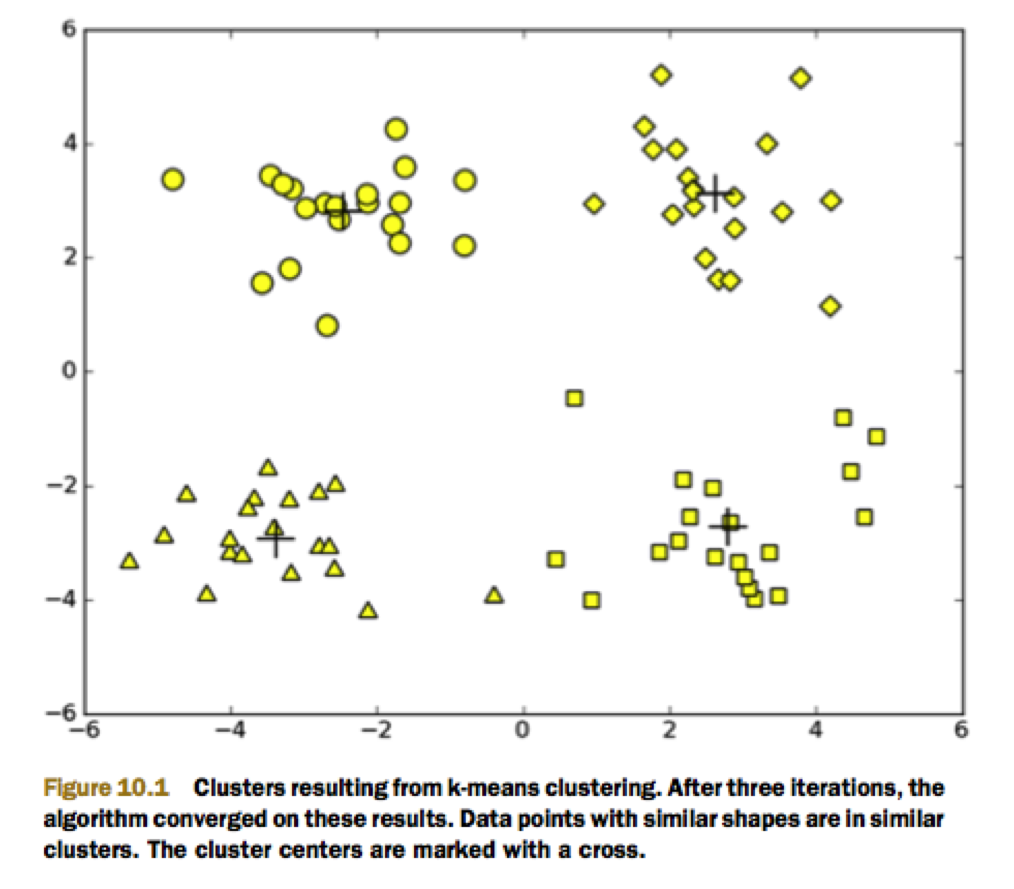
\includegraphics[width=1.0\textwidth]{fig10_1.png}
\caption{\label{fig:kmeans}Example of $K$-means clustering assignments.}
\end{figure}

$K$-means is the most famous clustering algorithm.  
It is a top-down, iterative, greedy approach that assumes vectorial data and finds a local optimum for \emph{K} cluster centers.  By \emph{top-down}, it means that \emph{k} is predetermined. By \emph{greedy}, it means that it is an approximation, and computing exact answers is prohibitively expensive. By \emph{local}, it means that it can get ``stuck'' on local extrema and therefore should always be run many times until stability is reached. By \emph{optimum}, it means that we can write down some cost function.
It depends heavily on averaging of vectors.  
Therefore, it assumes that all of the variables are quantitative, not categorical, as averaging categorical data doesn't make sense.

Assume we have $N$ observations of $p$-dimensional data denoted $x_{ij}$; $i=1,\ldots,N$; and $j=1,\ldots,p$.
$K$-means computes distances between data points using the Euclidean or $L_2$ norm:
$$
d(x_i, x_{i'}) = \sum_{j=1}^{p} (x_{ij} - x_{i\prime j})^2 = {\| x_i - x_{i'} \|}^2
$$
$K$-means assumes that the data is normalized, so the weights on all the features are the same. If feature stretching is desired, it should be done before running $K$-means.

Suppose we pick $K\ll N$ and choose cluster labels $k \in \{1, ..., K\}$.  
We assign each observation to exactly one cluster.  
We define a many-to-one mapping or ``encoder'' as $k=C(i)$, such that given the index of a data point, the encoder returns the cluster assignment of that point.

Would it be plausible to search over all possible encoders and pick the best one?  
In practice, that would be prohibitively expensive. 
The number of possible encoders is given by the Stirling number of the second kind:
$$
S(N,K) = \frac{1}{K!} \sum_{k=1}^{K} (-1)^{K-k} \binom Kk k^N
$$
For example, if $K=4$,
$S(10,4) = 34,105$.  
That's already quite large.  
$S(19,4) > 10^{10}$.  
Hence the brute force approach is not feasible.

K-means is a greedy, iterative approach. With its \emph{top-down}, \emph{greedy} and  \emph{iterative} (and online) approach, $K$-means examines a small subset of these possible encodings.  
To see how $K$-means works, first define the ``within-cluster'' point scatter as:
\begin{align*}
W(C) &= \frac{1}{2} \sum_{k=1}^{K}\sum_{C(i)=k}\sum_{C(i^\prime)=k} {\| x_i - x_i^\prime \|}^2 \\
&= \sum_{k=1}^{K} N_k \sum_{C(i) = k} {\| x_i - {\bar x_k} \|} ^2,
\end{align*}
where ${\bar x_k} = ({\bar x_{ik}}, \ldots, {\bar x_{pk}})$ is the mean vector of the $k$th cluster and $N_k = \sum_{i=1}^{N} I(C(i) = k)$ is the point count of the $k$th cluster.  
Given an encoder $C$, the within-cluster point scatter tells us how spread out the clusters are around their respective centroids. 
It does this by summing the squared norm of the distance between each pair of points within a cluster, or, equivalently, summing the squared norm of the distance from every point to the mean of the cluster and weighting it by the number of points in that cluster.

The purpose of the $K$-means algorithm is not classification, $K$-NN does the classification work.
The $K$-means algorithm (HTF Alg.~14.1) iterates the following 2 steps until the assignments stop changing.

\begin{enumerate}
\item Compute the means within each cluster given the current encoding $C$, call these $m_{1}$ ..., $m_{k}$.  
\item Reassign observations to closest cluster mean.
\end{enumerate} 
$$
C(i) = \underset{1 \leq k \leq K}{\arg\min} {\|x_i - m_{k} \|}^2
$$
The algorithm will start out with some sort of initialization for the means (pick random points from the data as initial means). 
We iterate until the many-to-one assignment changes stop. Which means the all the data points are already asssigned to closest cluster and there is no change in value for the computed cluster mean in successive iterations.
This is illustrated in Fig.~\ref{fig:kmeans} with $K=3$.
\begin{figure}
\centering
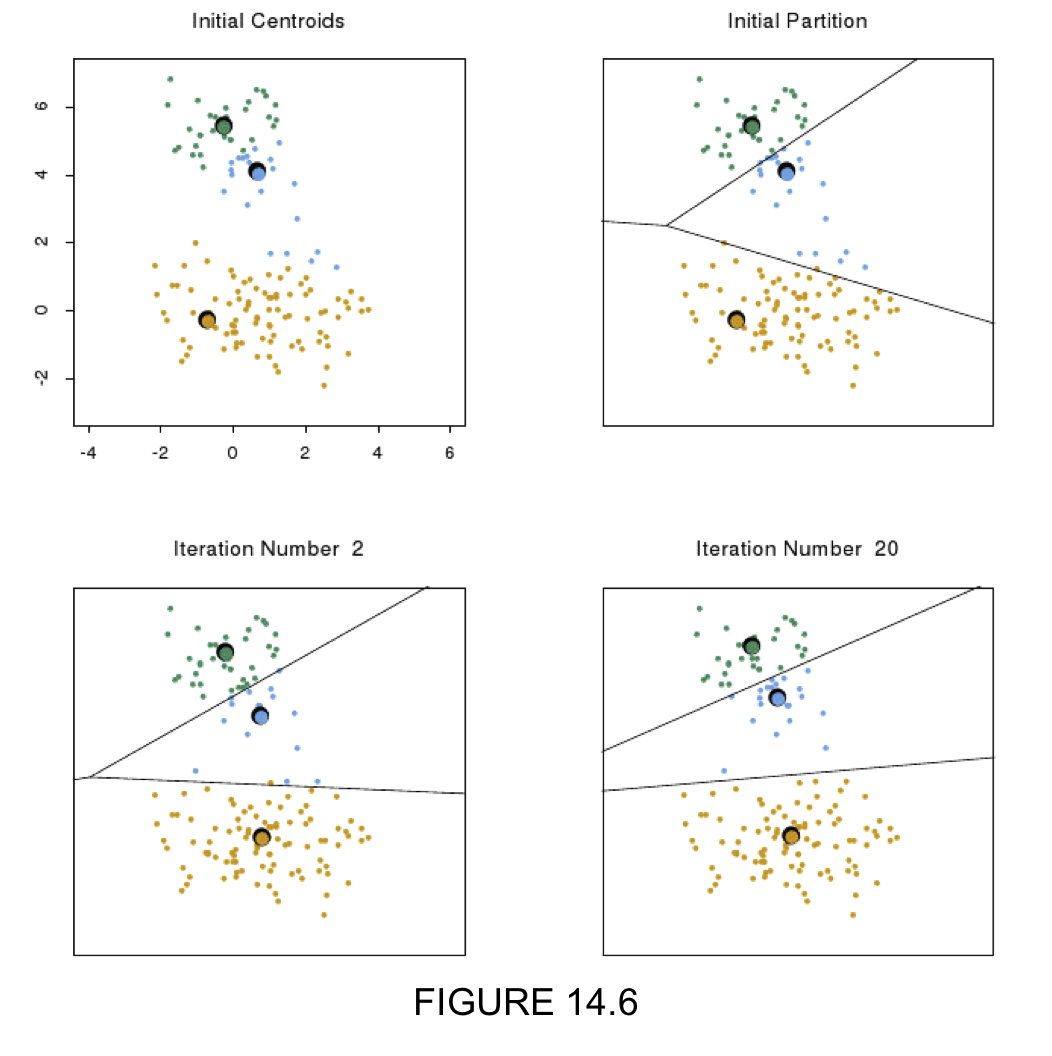
\includegraphics[width=1.0\textwidth]{fig14_6.png}
\caption{\label{fig:kmeans}Illustration of $K$-means clustering.}
\end{figure}

We can also look at this animated GIF of the $K$-means process starting in Fig. ~\ref{fig:kmeans_gif1}, ~\ref{fig:kmeans_gif3} and ending up in Fig. ~\ref{fig:kmeans_gif2}, ~\ref{fig:kmeans_gif4}. \href{https://f.hypotheses.org/wp-content/blogs.dir/253/files/2015/02/k-means-5-pts-3B.gif}{(Link to GIF)}


\begin{figure}
\centering
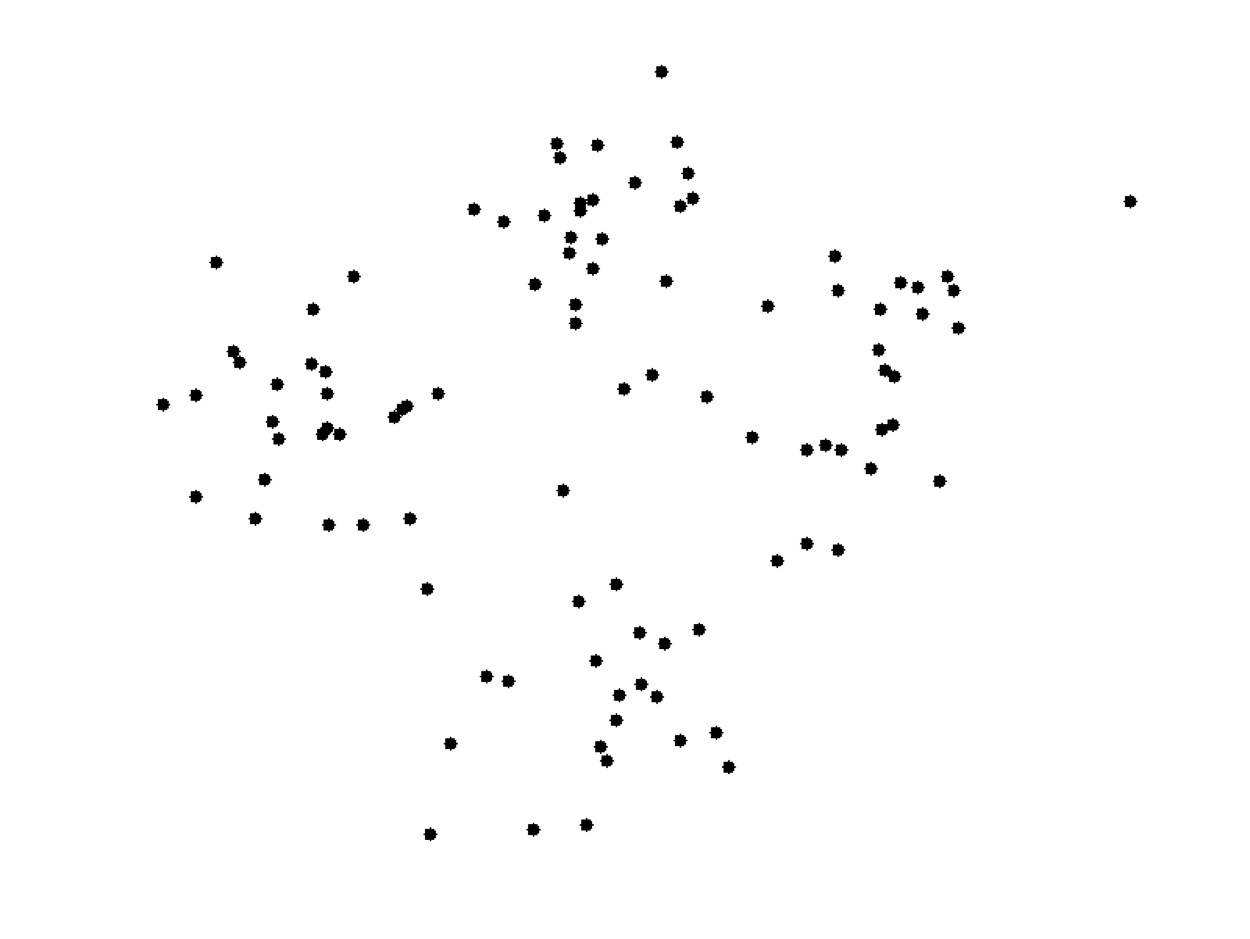
\includegraphics[width=1.0\textwidth]{points.png}
\caption{\label{fig:kmeans_gif1}Before $K$-means clustering (example 1)}
\end{figure}

\begin{figure}
\centering
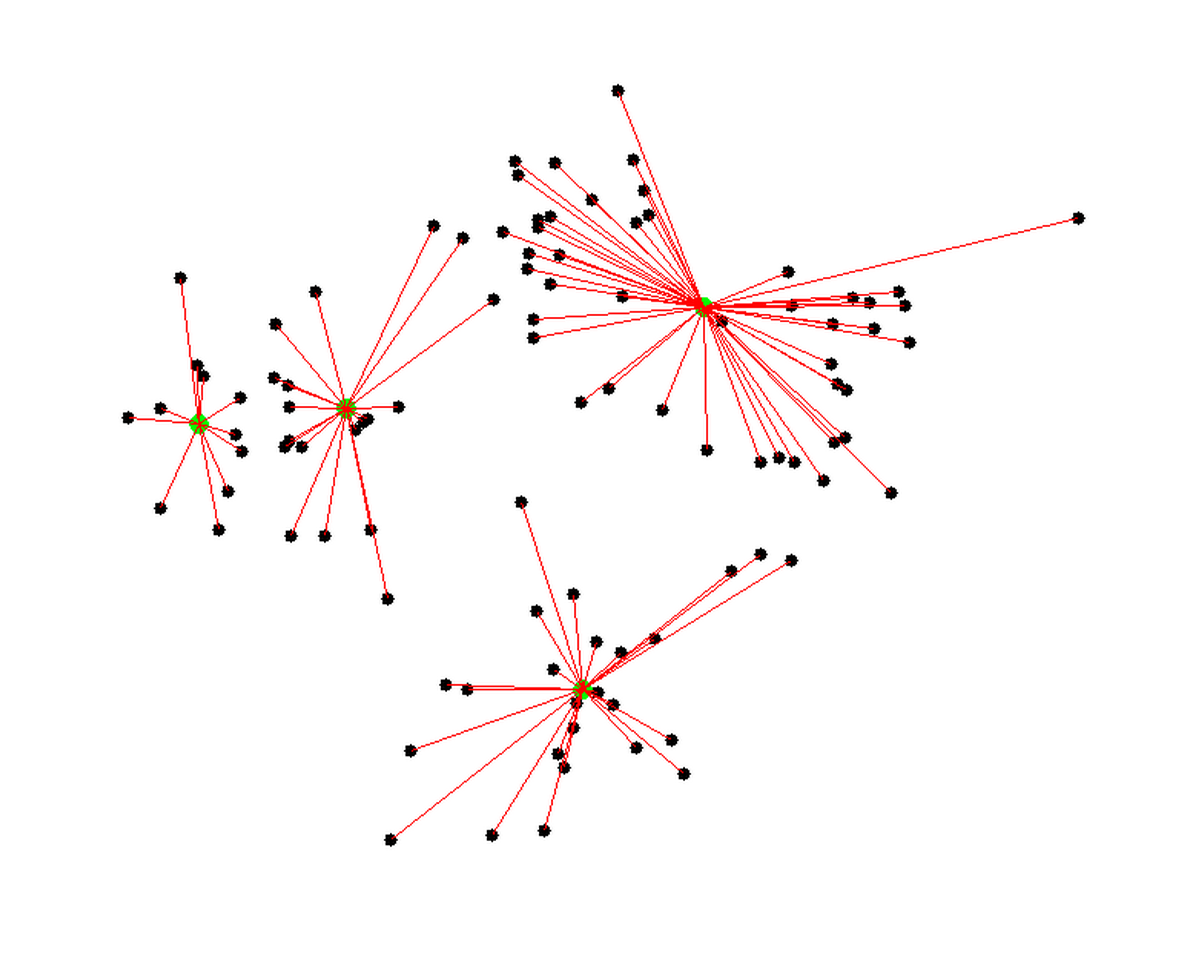
\includegraphics[width=1.0\textwidth]{points_done.png}
\caption{\label{fig:kmeans_gif2}Completed $K$-means clustering (example 1)}
\end{figure}

\begin{figure}
\centering
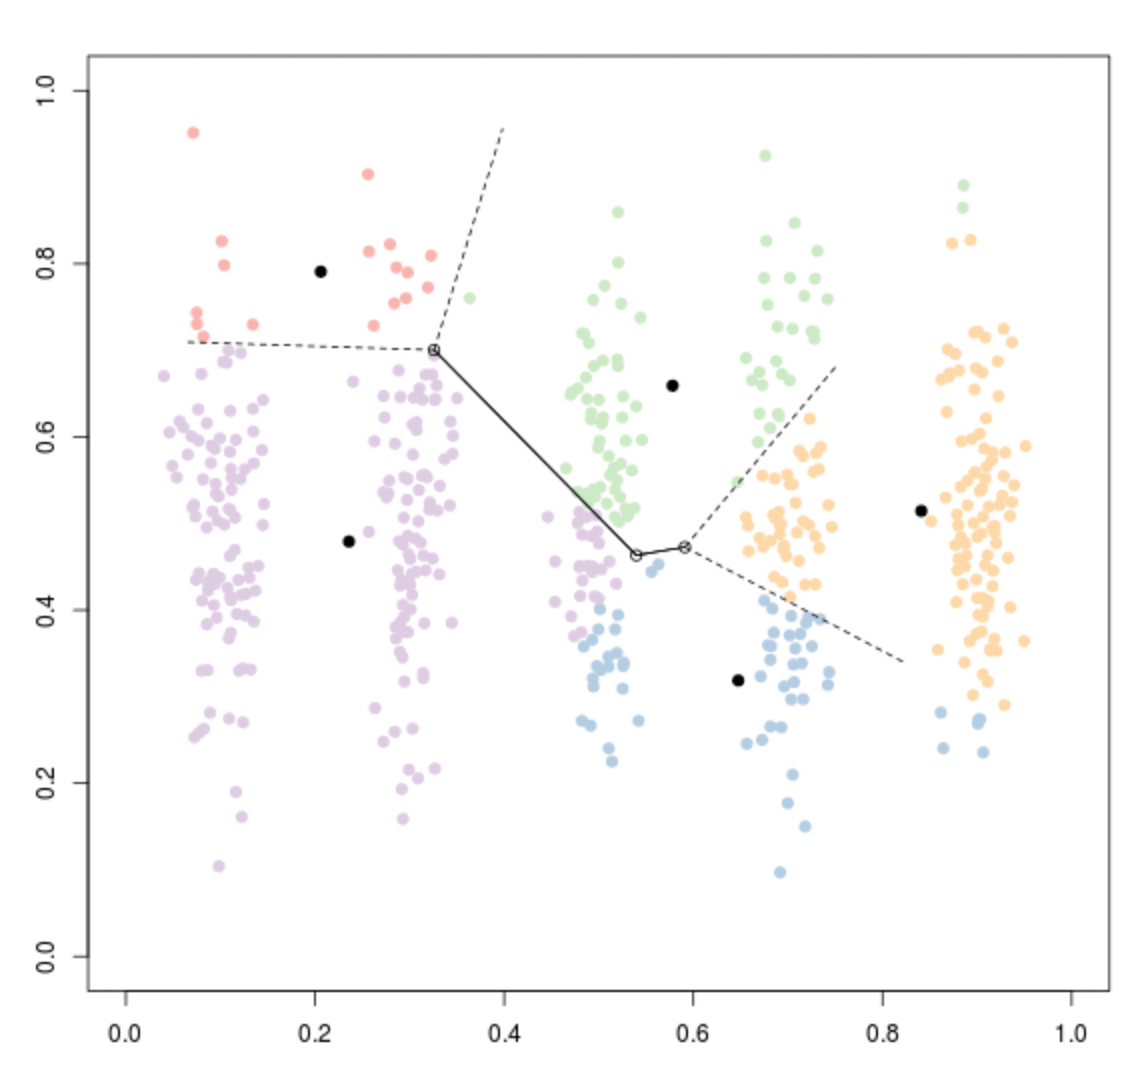
\includegraphics[width=1.0\textwidth]{visualize0.png}
\caption{
\label{fig:kmeans_gif3}Before $K$-means clustering (example 2)}
\end{figure}

\begin{figure}
\centering
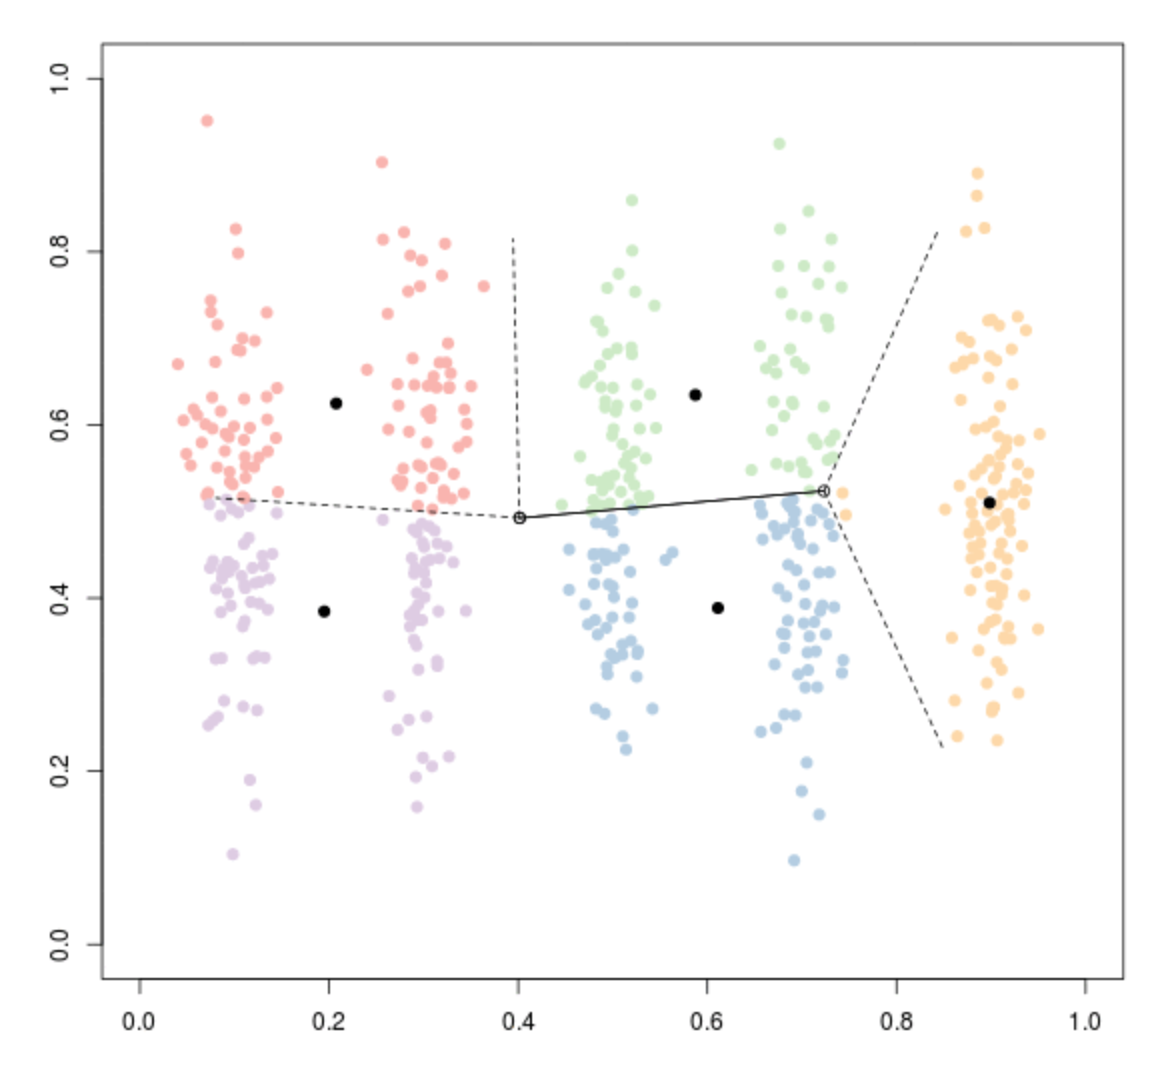
\includegraphics[width=1.0\textwidth]{visualize1.png}
\caption{\label{fig:kmeans_gif4}Completed $K$-means clustering (example 2)}
\end{figure}


One way to stop is when the labels stop changing.  
However, this can be tricky if labels keep flip-flopping.  
One alternative is to stop if the cluster centers or overall cost stop changing according to some threshold.  
Or, you could just stop after a fixed number of iterations.

When faced with a tie, we can just choose the cluster arbitrarily as we will run the process many times.

Note that K means will always converge in finite time. Also we may not reach global optima as the algorithm may converge to a local optima. 

How do we choose $K$?  

There is no optimal $K$. Since this is an unsupervised problem, we can't use cross validation to choose $K$ (the class label assigned here has no meaning and for each time, it can be of different label).  
You should definitely try a number of different initializations for each $k$ (maybe 30), as the algorithm may not find the same partitions each time.  
You could use some heuristic of how often the same partitions (for example, whether two points are assigned in the same cluster) are formed with different initializations.  
If this wasn't stable you could change $K$.  

This is an instance of a \emph{model order selection problem} in machine learning since adding $K$ will always reduce error.  
If $K$ becomes $N$, it can achieve $0$ error, but that isn't very useful.  
Naturally, we need to find a compromise between cost and complexity.    
There are a variety of information-theoretic or stability-based heuristics one can use for choosing $K$, but again, there is no single correct value of $K$, just nice heuristics.

Recall: $K$-NN is used for classification or regression and is supervised. $K$-means is for clustering and is unsupervised.

\subsection{Fitting Gaussian Mixtures}
As we saw above, $K$-means uses hard cluster assignment on each iteration, so cluster memberships are popping back and forth.  
Gaussian mixture models (GMM) fitting using the Expectation-Maximization (EM) algorithm offer a soft alternative to $K$-means.  
We'll go through the process of GMM fitting using EM for $K=2$ and $p=1$ and see how that reduces to $K$-means.  
With $K=2$ we have a bimodal distribution specified as follows:
$$
Y_1 \sim \mathcal{N}(\mu_1, \sigma_1^2),\quad Y_2 \sim \mathcal{N}(\mu_2, \sigma_2^2)
$$
and
$$
Y = (1-\Delta)Y_1 + \Delta Y_2 \quad \text{with}\quad \Delta \in \{0,1\}, \; Pr(\Delta=1) = \pi.
$$
You flip a coin with probability $\pi$ that delivers outcome $Y_1$ or $Y_2$.  
This is a \emph{generative representation}.  
We don't get to observe $Y_1$ or $Y_2$ directly since it's unobserved -- we can only observe $Y$, which we model as the outcome of a random experiment. The outcome of the random experiment, denoted here by $\Delta$, is a \emph{latent variable}.

Sometimes, it is better to tie the variances together to avoid over-fitting and lower costs.

For instance, if we were measuring blood sugar for diabetes we would probably see a bimodal distribution with a histogram.  
But, we don't know what the labels are.  We just want to see if there's a cluster structure in the data. The coin-flipping and specified distribution would generate the random data for us.

Let $\phi_\theta(x)$ denote the normal density with parameters $\theta = (\mu, \sigma^2)$.  
We can write the density of $Y$ as
$$
g_Y(y) = (1 - \pi)\phi_{\theta_{1}}(y) + \pi\phi_{\theta_{2}}(y)
$$
We want to fit this model to a dataset of $N$ samples, i.e.,  to solve for the parameters $\theta = (\pi, \theta_1, \theta_2) = (\pi, \mu_1, \sigma_1^2, \mu_2, \sigma_2^2)$.  
The log-likelihood is given by
$$
\ell(\theta;Z) = \sum_{i=1}^N \log[(1-\pi)\phi_{\theta_{1}}(y_i) + \pi \phi_{\theta_{2}}(y_i) ]
$$
where $Z$ denotes the observed data.  
Direct maximization of this log likelihood is hard due to the sum of terms in the log.  
Instead, let's pretend we know the value of the latent variable $\Delta$ for each point and write:
$$
\ell_0(\theta; Z, \Delta) = \sum_{i=1}^N [(1-\Delta_i) \log \phi_{\theta_{1}}(y_i) + \Delta_i \log \phi_{\theta_{2}}(y_i)] + \sum_{i=1}^N [(1-\Delta_i) \log (1-\pi) + \Delta_i \log \pi]
$$
Then we can estimate $\mu_1$ and $\sigma_1^2$ from the sample mean and variance for the data with $\Delta_i = 0$, similarly for $\mu_2$ and $\sigma_2^2$ when $\Delta_i=1$. 
We estimate $\pi$ from the proportion for which $\Delta_i =1$.

Of course, we don't actually know the $\Delta_i$s.  
We address this problem by making a guess and iterating as follows.  
For each $\Delta_i$ above, we substitute its expected value.
$$
\gamma_i(\theta) = E(\Delta_i | \theta, Z) = Pr(\Delta_i = 1 | \theta, Z)
$$
This is also known as the \emph{responsibility} of the model (model 2, in this case) for observation $i$.  
The responsibility for model 1 would be 1 minus this, since there are only two components.

The EM Algorithm (HTF 8.1) for a bimodal GMM is as follows (it looks pretty familiar):
\begin{enumerate}
\item Take initial guesses for $\hat{\mu}_1,\hat{\sigma}_2^2,\hat{\mu}_2,\hat{\sigma}_2^2,\hat{\pi}$
\item E-step: compute responsibilities \\
$$
\hat{\gamma_i} = \frac{\hat{\pi}\phi_{\hat{\theta}_2}(y_i)}{(1-\hat{\pi}) \phi_{\hat{\theta}_1}(y_i) + \hat{\pi} \phi_{\hat{\theta}_2}(y_i)} \quad \text{for} \quad i=1,...,N
$$
\item M-step: compute weighted means and variances
\begin{align*}
\hat{\mu}_1 &= \frac{\sum_{i=1}^{N} (1-\hat{\gamma_i})y_i}{\sum_{i=1}^{N} (1-\hat{\gamma_i})}  \\
\hat{\sigma}_1^2 &= \frac{\sum_{i=1}^{N} (1-\hat{\gamma_i})(y_i-\hat{\mu}_1)^2}{\sum_{i=1}^{N} (1-\hat{\gamma}_i)}
\end{align*}
and similarly for $\hat{\mu}_2$, $\hat{\sigma}^2_2$ using $\hat{\gamma}_i$ in place of $(1-\hat{\gamma}_i)$.  The mixing probability is given by $\hat{\pi} = \sum_{i=1}^{N} \frac{\hat{\gamma_i}}{N}$.

\item Iterate steps 2 and 3 until convergence.

\end{enumerate}

Fig.\ \ref{fig:gmm_1} shows an example.  
The histogram on the left gives us a rough idea that the data is bimodal.  
We start  with guesses for the means and variances for the two Gaussian components, compute the responsibilities, then compute weighted means and variances conditioned on the current responsibilities and iterate.  
The green curve on the right represents the responsibilities to one of the modes.  
In EM, the responsibilities lie in a continuum from 0 to 1.  This means that membership is "soft" compared to \emph{K} means where membership is either 0 or 1.
Only the responsibility for the first mode is shown since the other one is one minus it.  
For every tick mark along the bottom, the dots on the green curve show the responsibility for the first mode.  
The averaging takes every data point into account but weights them by the responsibility.  
Because the responsibility drops off so fast, you probably aren't taking many of the right points into account for the first mean and variance.
Fig.\ \ref{fig:gmm_2} plots the log-likelihood as a function of iteration.  
It appears to be heading into a plateau, which suggests a criterion for stopping.


\begin{figure}
\centering
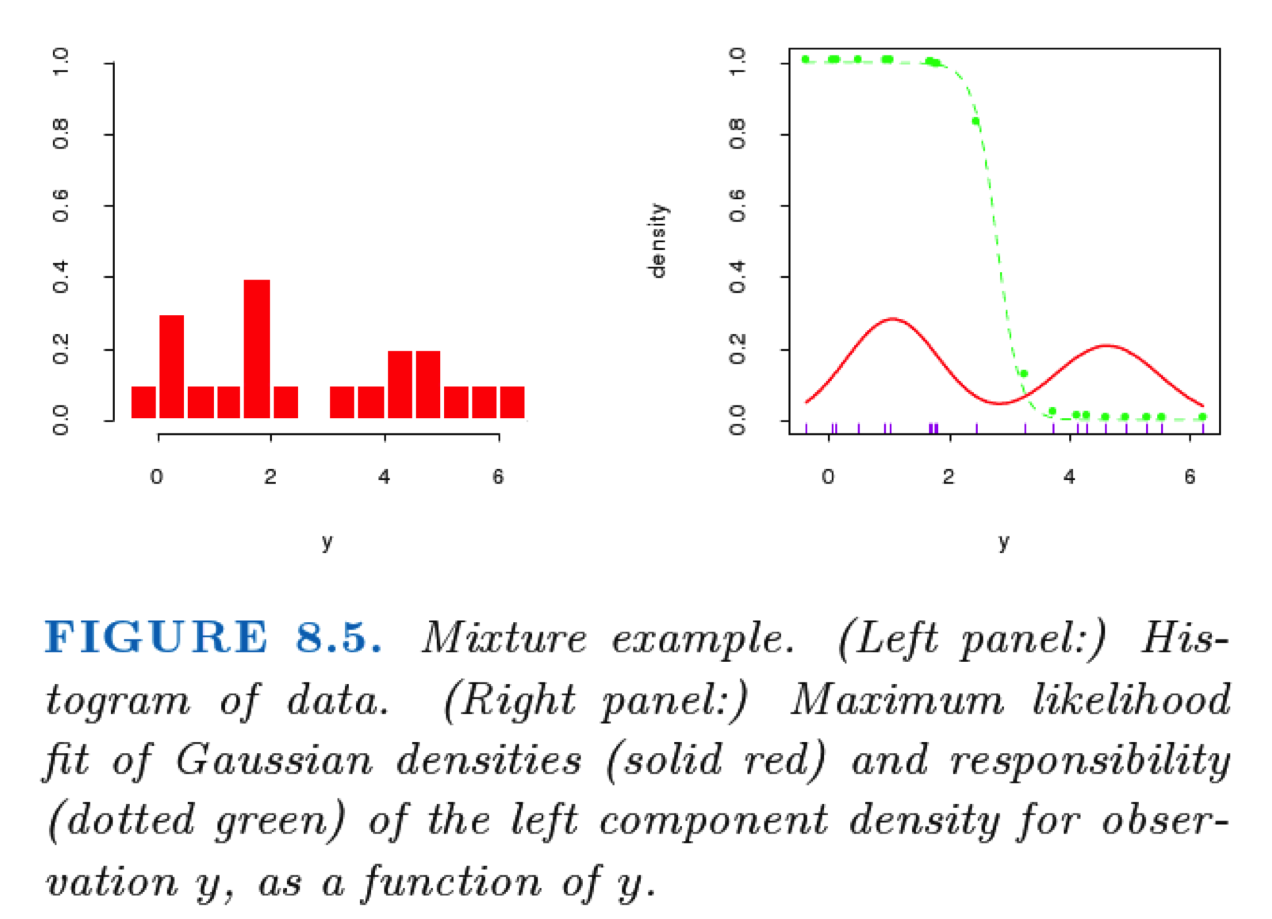
\includegraphics[width=0.8\textwidth]{fig8_5.png}
\caption{
	\label{fig:gmm_1}
    Example of Gaussian Mixture Model fit.
}
\end{figure}

\begin{figure}
\centering
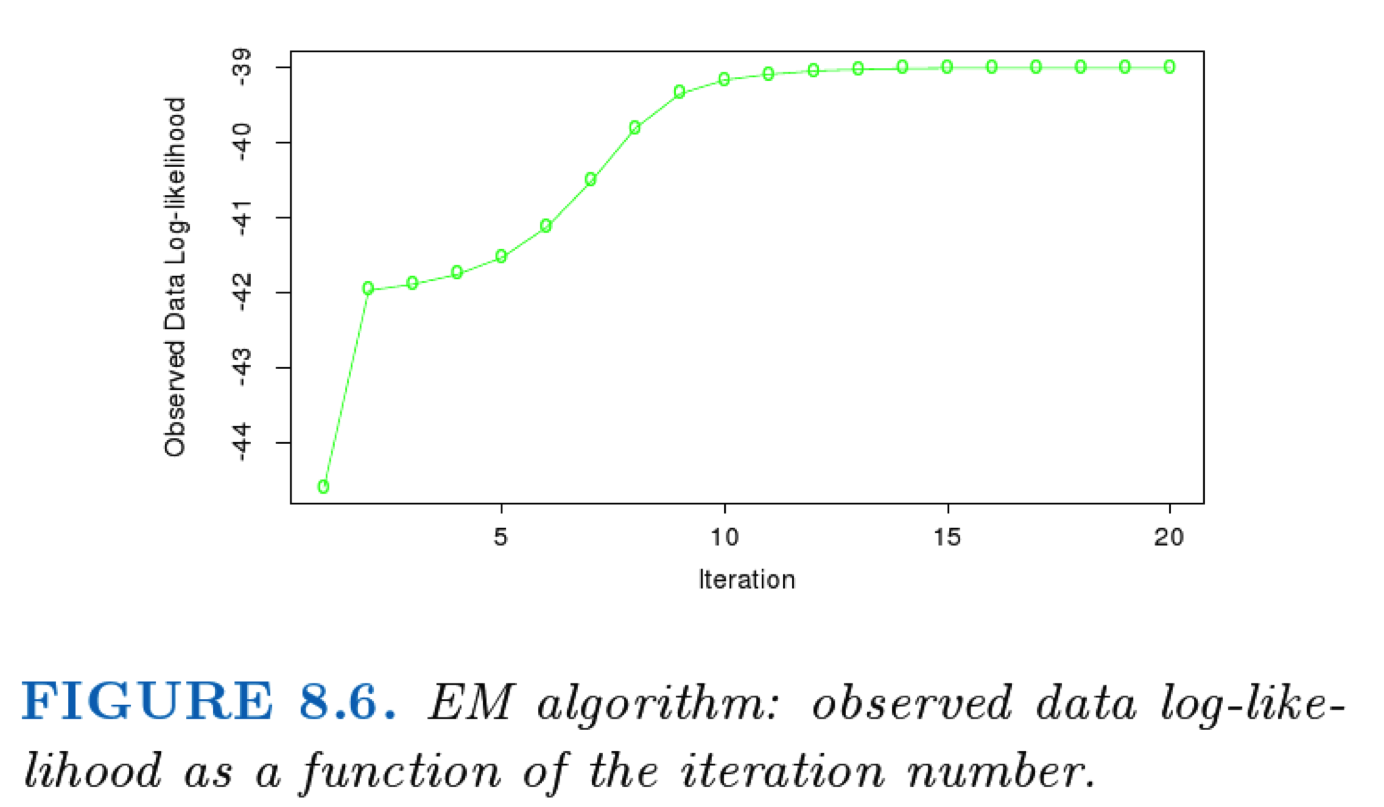
\includegraphics[width=0.8\textwidth]{em_alg.png}
\caption{
	\label{fig:gmm_2}
    Log-likelihood vs.\ iterations of EM.
}
\end{figure}

Fig.\ \ref{fig:gmm_3} shows an example from scikit-learn that, like the above example, is bimodal, but in this case the data is 2D instead of 1D.  
This requires a slight change to the maximization step to compute the mean vector and covariance matrix instead of the scalar mean and variance.   
When applying EM to GMM fitting when $p>1$, we have the option of using a full, diagonal or spherical covariance matrix.  
Spherical means the covariance matrix has the form $\sigma^2 I$ where $I$ is a $p\times p$ identity matrix.  
In this example, the covariance matrices are full, and we see that they have adapted to the spread of the data in each mode.

\begin{figure}
\centering
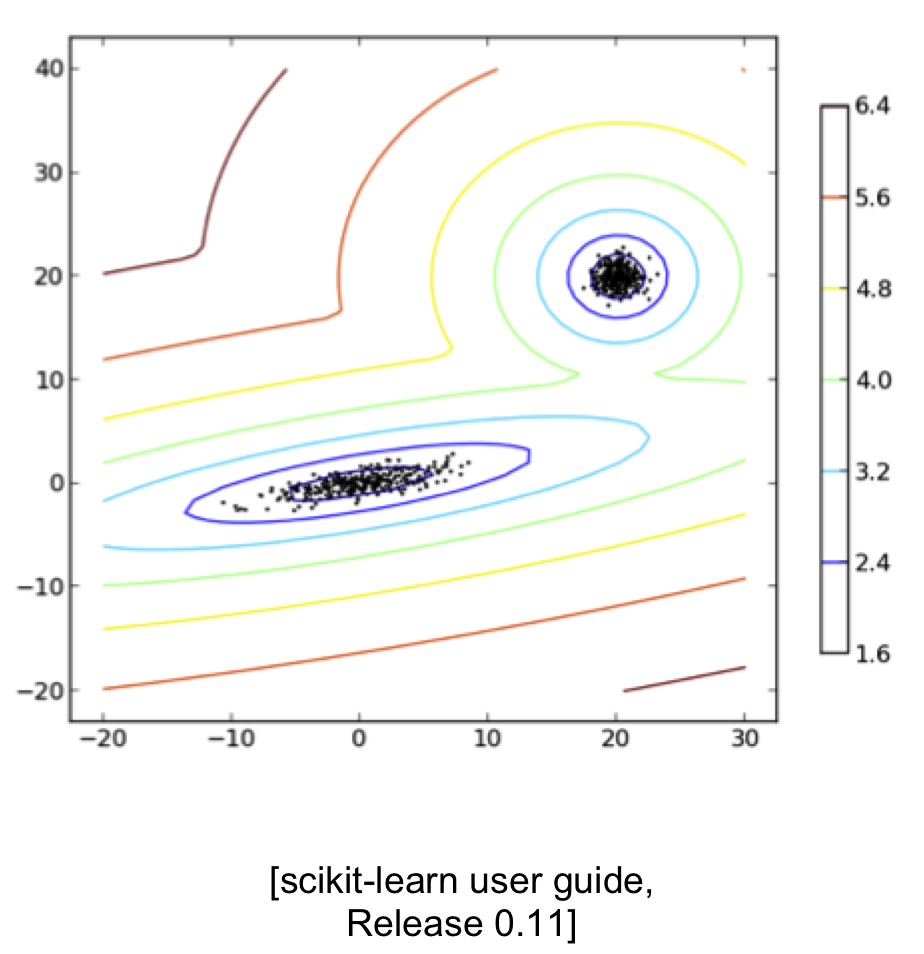
\includegraphics[width=0.8\textwidth]{scikit.png}
\caption{
	\label{fig:gmm_3}
    Scikit learn example.
}
\end{figure}

Finally, in Fig.\ \ref{fig:gmm_4} we connect GMM/EM fitting  to $K$-means.  
If you set all covariance matrices to $\sigma^2 I$ (i.e., spherical) and drive $\sigma^2$ to 0, this produces hard assignments.  
Therefore, when we run $K$-means,g it's as if we're doing GMM with EM but instead of letting each cluster have its own covariance matrix, they all have to be round covariance matrices and we make $\sigma^2$ tiny so there's no longer any notion of shared membership between clusters.  

As a side note, $K$-means is sometimes used to initialize GMM/EM fitting.

\begin{figure}
\centering
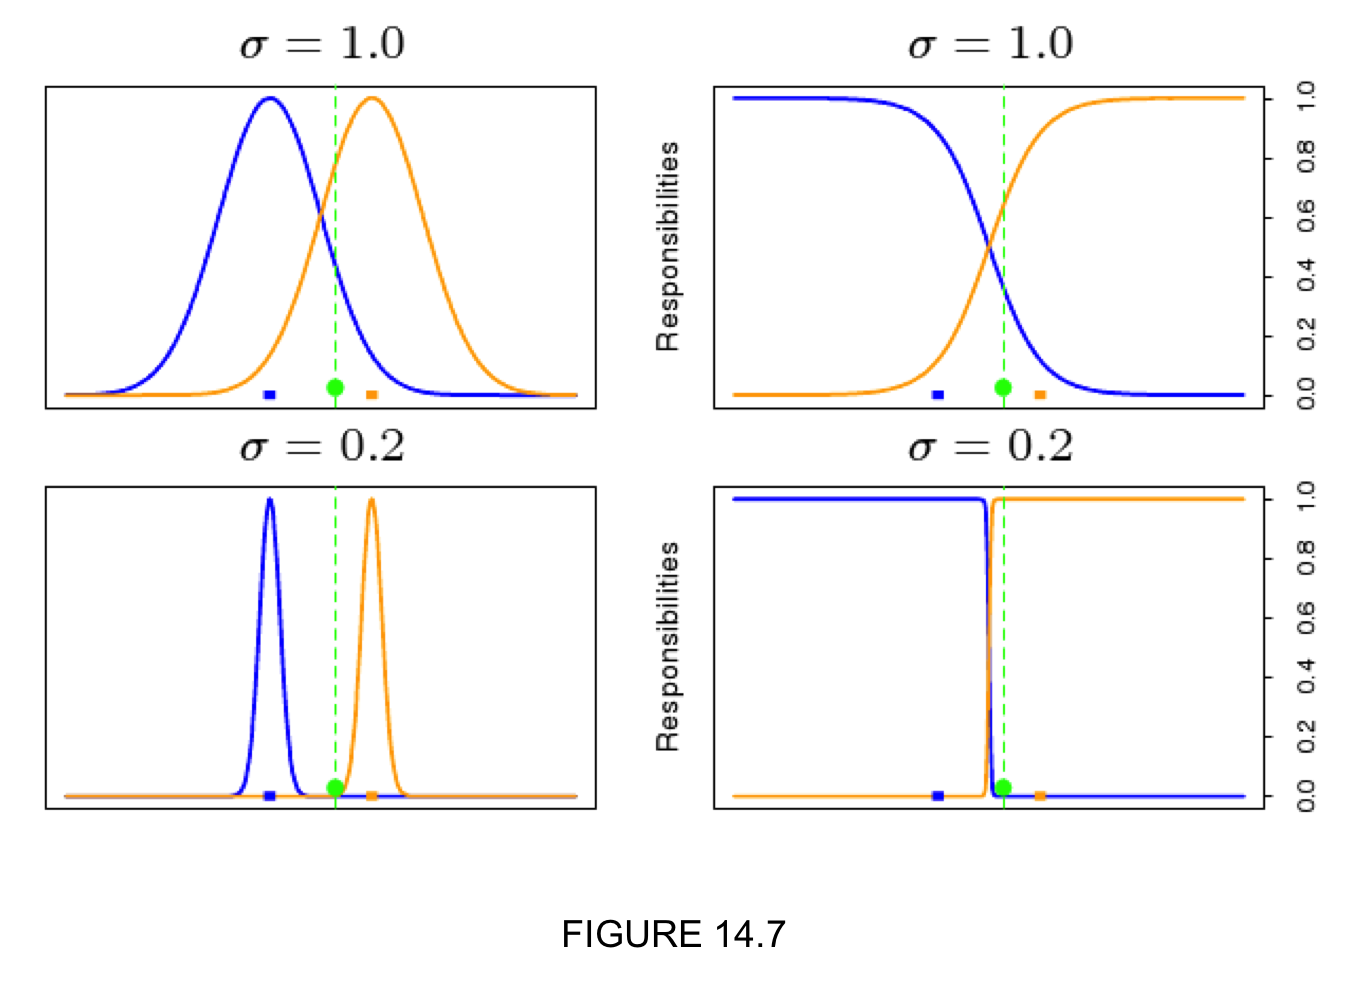
\includegraphics[width=0.8\textwidth]{fig14_7.png}
\caption{
	\label{fig:gmm_4}
	Left: Gaussian densities for two modes with the same means but different variances.  
	Right: plot of responsibilities.  
    In the case where $\sigma=1.0$ the green dot picks off shared responsibilities between the two modes.  
    When $\sigma=0.2$ the green dot gets a responsiblity of nearly 1 for the right mode and nearly 0 for the other since it lies just a hair to the right of the midpoint between the two means.  
}
\end{figure}

\end{document}
